% Scalar instruction entry source: tools/generate_scalar_instruction_catalog.py.
\subsection{\texttt{DC.IALL}}
\label{sec:scalar-dc_iall}
\index{DC.IALL@\texttt{DC.IALL}}
\begin{sloppypar}\noindent\textbf{Purpose.} Invalidates all data-cache state defined by the scalar profile.\end{sloppypar}\smallskip
\noindent\textbf{Syntax.}\par
\begin{lstlisting}[style=ptoscalarcode]
dc.iall
\end{lstlisting}
\noindent\textbf{Encoding.}\par
\noindent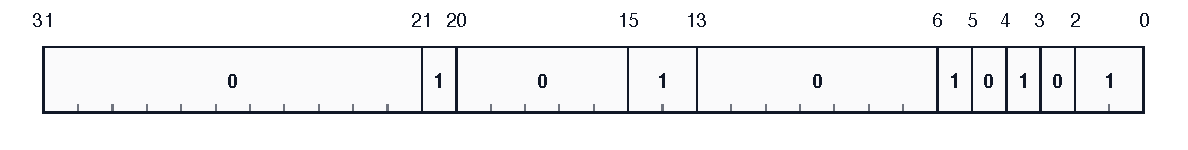
\includegraphics[width=\textwidth]{figs/encoding/scalar_instruction_entries/enc_dc_iall.pdf}\par\smallskip
\begin{description}[leftmargin=0.18\linewidth,style=nextline]
\item[Format] \texttt{L32} \texttt{32-bit} scalar word.
\item[Pattern] \texttt{00000000000100000110000000101011}.
\end{description}
\noindent\textbf{Classification.}\par
\begin{description}[leftmargin=0.18\linewidth,style=nextline]
\item[Category] System, Cache, SSR, and Execution Control.
\item[Family] Cache Maintain.
\item[Execution class] \texttt{SYS}; uop\_kind=SYS, sys\_kind=CACHE\_MAINT.
\end{description}
\noindent\textbf{Operand fields.}\par
\noindent No variable operand fields are present in this fixed encoding.\par\smallskip
\noindent\textbf{Operation.}\par
\begin{lstlisting}[style=ptoscalarcode]
Maintain(op)
\end{lstlisting}
\Needspace{0.08\textheight}
